\documentclass[10pt,a4paper]{book}
\usepackage[italian]{babel}
\usepackage[utf8]{inputenc}
\usepackage{amsmath}
\usepackage{amsfonts}
\usepackage{amssymb}
\usepackage{graphicx}
\usepackage{float} 
\begin{document}

\chapter{Introduzione}
\section{Argomenti}
\begin{itemize}
\item Agenti intelligenti;
\item Problemi e algoritmi di ricerca;
\item Giochi con problemi di ricerca: siano negli anni '70 dove si ispezionano tutti i casi possibili con un agente intelligente.
\item Rappresentazione della conoscenza e ragionamento: dagli anni '70 in poi. Il calcolo proposizionale risulta non sufficientemente espressivo, ma permette di fare inferenza (conoscenza). Si parla di calcolo dei predicati e di programmazione logica. Si ottiene in questo modo una definizione del problema e del dominio che porta a ottenere un risultato del problema.
\item Trattazione dell'incertezza: nel mondo reale esiste il problema dell'incertezza, diversi gradi modellati abbastaza bene con la teoria di probabilit\`a. L'incertezza si risolve conoscendo la distribuzione di probabilit\`a congiunta. Ovvero indipendenza condizionale dove, per esempio, se conosco C, allora A \`e indipendente da B (fattorizzazione della probabilit\`a congiunta). Esperessione nelle reti \textit{bayesiane}.
\item Introduzione all'Apprendimento automatico, \textit{Machine Learning} e Apprendimento con rinforzo: va considerato come usare un modello probabilistico ha un costo computazionale enorme. Per questo nasce l'Apprendimento automatico, ovvero quando l'elaboratore acquisisce informazioni per avere conoscenza mediante addestramento. Nelle Reti Neurali si superano le prestazioni dell'essere umano nel riconoscimento di suoni, parlato, elaborazione dati, .. .
In ogni caso c'\`e sempre necessit\`a di una grande potenza computazionale e dati. Per questo i maggiori \textit{leader} in tali ambiti sono Google, IBM e Microsoft.
\\
Tuttavia l'aumento della potenza dell'elaboratore non porta buoni risultati solo nell'area dell'apprendimento, ma anche della probabilit\`a.\\
Si parla di apprendimento con rinforzo quando vengono provate \textit{random} tutte le strade possibili, concetrandosi per avere risultati su quelle migliori.
\item Elaborazione linguaggio naturale: \`e il linguaggio naturale che permette ai \textit{robot} di comprendere e interagire con il mondo esterno;
\item Visione aritificiale.
\end{itemize}

\section{Agente intelligente}
Un agente razionale \`e un agente intelligente.\\
Esistono tanti tipi di intelligenza: emotiva, relazionale, ecc.\\
Un agente agisce nel mondo che lo circonda, ha degli obiettivi fissati che raggiunge per mezzo dell'informazione che ha disponibile.\\
Incide la potenza di calcolo, percui un agente \`e intelligente se riesce a fare il suo meglio possibile, anche solo avvicinandosi a dei risultati.\\
Cerca di massimizzare il soddisfacimento dei propri bisogni sfruttando le informazioni di cui dispone, o che pu\`o acquisire per mezzo delle sue azioni.\\
Dal punto di vista matematico usa tempi discreti come momento di acquisizione delle informazioni, ed \`e  formalizzabile come:
\begin{equation}
f:\textit{P*} \longrightarrow \textit{A}
\end{equation}
dove f rappresenta un obiettivo e $\longrightarrow$ tutte le informazioni possibili per poter raggiungere quell'obiettivo.\\
Tuttavia le limitazioni computazionali possono impedire la realizzazione di razionalit\`a perfetta, dunque si cerca esempio di usare la memoria a disposizione nel modo migliore.\\
Gli agenti si distinguono in agenti fisici, come \textit{robot}, attuatori, umani e \textit{soft}, come il contenuto di una pagina \textit{web}.\\
Il dominio di f rappresenta tutte le possibili percezioni da quando l'agente ha iniziato a funzionare.
\\\\
Esempio dell'aspirapolvere: deve sapere dove si trova e se la stanza \`e sporca.\\
Percezioni: stanza, pulito/sporco.\\
Azioni: sinistra, destra, aspira.\\
\\
L'algoritmo non \`e intelligentissimo, perch\`e se le stanza sono tutte pulite continua ad andare avanti e indietro, per\`o tale algoritmo fa uso di pochissima memoria.\\
Importante \`e fissare la misura di prestazione che valuta la sequenza di percezioni, ovvero quanto bene ha lavorato il robottino con un certo numero di risorse. Inoltre non \`e detto che il robottino aspiri sempre tutto, per questo la misura dipende anche dalle caratteristiche dell'ambiente.
Lo scopo \`e individuare la misura di prestazione massimizzata. Per farlo non \`e necessario che l'agente sia omniescente, basta che sia razionale e faccia del suo meglio con le informazioni. Razionalit\`a non \`e sempre sinonimo di successo (per mancanza di risorse, esempio precisione non disponibile).\\
Inoltre un agente razionale deve saper anche risolvere situazioni che il progettista non ha pensato, grazie all'addestramento.\\
\\
PEAS identifica 4 componenti da caratterizzare, le caratteristiche dell'ambiente dove l'agente \`e chiamato a operare: la misura delle prestazioni, l'ambiente operativo, attuatori (le percezioni) e i sensori (le azioni). 

\subsection{Pilota automatico per taxi}
\begin{itemize}
\item \textbf{Misura di prestazione}: obiettivi che si intendo realizzare, arrivare a destinazione corretta, profitto massimo, veloce, ligio alla legge, viaggio confortevole.
\item \textbf{L'ambiente}: in cui l'agente deve operare, strade, altri veicoli, pedoni, clienti;
\item \textbf{Attuatori}: reagiscono verso l'ambiente, acceleratore, sterzo, freno, frecce, clacson, schermo di interfaccia per comunicare con i passageri.
\item \textbf{Sensori}: recepiscono informazioni dall'ambiente, permettendogli di raggiungere i suoi obiettivi, telecamere, \textit{sonar}, tachimetro, GPS contachilomeri, accelerometro, sensori sul motore, tastiera.
\end{itemize}
\noindent
Per progettare un agente devono essere fatte delle scelte:
\begin{itemize}
\item \textbf{Osservabile}: quando i sensori hanno accesso allo stato completo dell'ambiente in ogni momento. I sensori devono essere in grado di misurare gli aspetti rilevanti per le scelte dell'azione. Altrimenti si parla di osservabilit\`a parziale o non osservabile.
\item \textbf{Deterministico}: lo stato successivo \`e completamente determinato dallo stato corrente dell'agente, in caso contratio si parla di stocasticit\`a.
\item \textbf{Episodico}: esperienza dell'agente che non deve dipendere da episodi precedenti, altrimenti si parla di sequenziale. In ambienti episodici la scelta dell'azione dipende esclusivamente dall'episodio corrente
\item \textbf{Statico}: l'ambiente \`e stazionario nel tempo, altrimenti parliamo di ambiente dinamico.
\item \textbf{Discreto}: applicato allo stato dell'ambiente, il modo in cui \`e gestito il tempo, alle percezioni e azioni dell'agente. \`E discreto quanto si ha un numero finito e distinto. Discreto quando i punti sono successivi l'uno all'altro.
\item \textbf{Agente}: numero di agenti presenti nell'ambiente, con il vincolo che l'agente B ha un comportaento che tenta di massimizzare una misura di prestazione da cui dipende il comportamento di A.
\end{itemize}
\subsection{Tipi di agenti}
Un agente ha sensori e attuatori
\subsubsection{Agenti a riflesso semplice}
Si dimentica la storia, si ricorda solo l'ultima percezione percepita. Prende la decisione sull'azione da compiere solo sulla base di quello percepito al tempo T.\\
Per realizzare l'agete basta soddisfare la relazione condizione soddisfatta $\rightarrow$ azione conseguente. Un esempio \`e quello dell'aspirapolvere.
Sulla base delle informazioni percepite dai sensori, si seleziona la regola, dunque l'azione da svolgere con gli attuatori.\\
Tuttavia vi \`e un problema. Se l'ambiente \`e parzialmente osservabile, l'agente pu\`o fallire. Se, difatti, cambia qualche situazione di contorno si pu\`o ritrovare all'interno di un \textit{loop} (come nel caso di un ragnetto in un labirinto portato sempre a sinistra e poi per qualche motivo si trova a dover svoltare a destra). A tale inconveniente si pu\`o reagire con una scelta \textit{random}.\\
In conclusione con un agente a riflesso semplice si hanno delle regole fissate e un unico \textit{goal}.

\subsubsection{Agenti a riflesso con stato}
Nasce come miglioramento alla tipologia di agente precedente. Si tiene traccia, in memoria, delle percezioni passate. \`E per\`o osservabile solo se l'ambiente \`e statico. In questo modo si crea una mappa come modello di come il mondo evolve e l'effetto delle singole azioni nel mondo.\\
In questo caso nella sequenza condizione $\rightarrow$ azione \`e incluso anche lo stato che permette di lavorare anche in ambienti parzialmente osservabili.\\
Tuttavia tale approccio \`e ancora poco flessibile, perch\`e il comportamento degli attuatori rimane nelle regole che permettono di raggiungere un certo \textit{goal}. Tale tipologia ha portato il vantaggio di togliere le limitazioni alle regole.
\subsubsection{Agenti basati su goal}
Definisco degli obiettivi internamente che permettono la selezione dell'azione da parte degli attuatori. Viene svolta una sorta di simulazione di cosa dovrebbe succedere per uno specifico \textit{goal} in modo da selezionare le azioni che portano al suo soddisfacimento.
\subsubsection{Agenti basati su una misura di utilit\`a}
In questo caso l'agente ha una misura di utilit\`a. Tale funzione serve quando un'agente ha pi\`u obiettivi che non possono convivere e dunque deve seleziona quale privilegiare o a valutarne la probabilit\`a di successo. Nel concreto la funzione utilit\`a  assegna a uno stato un numero reale che \`e la contentezza a esso associato.
Questo porta un agente basato sugli obiettivi a assumere comportamenti di alta qualit\`a. Per esempio nel caso del taxi ci sono molte strade che portano alla stessa destinazioni ma alcune sono pi\`u sicure, pi\`u veloci, affidabili, economiche.
\\\\
\noindent
Ogni architettura risponde ad agenti diversi a seconda del compito da svolgere.
\\\\
Gli agenti possono anche apprendere, questo \`e possibile innestarlo su ogni tipo di agente. L'apprendimento suggerisce delle modifiche alle componenti interne delle architetture, in base a quello appreso fino a quel momento. In questo modo si ha un aggiornamento costante di regole e azioni. Per esempio sulla base del \textit{goal} l'agente pu\`o apprendere se il mondo \`e continuo o stocastico, e cos\`i fare delle stime sulle azioni.\\
All'interno di un'architettura di apprendimento si trovano due componenti importanti:
\begin{itemize}
\item \textbf{\textit{Critic}}: che si occupa di valutare il risultato ottenuto da un'azione, e nel caso non sia buono continuare;
\item \textbf{\textit{Problem generator}}: che mitiga il rischio di sovraspecializzazione, ovvero l'apprendimento solo su una certa parte del dominio. Il \textit{Problem generator} forza l'agente a esplorare tutte le possibilit\`a dell'ambiente.
\end{itemize}
\newpage
\chapter{Risoluzione di problemi}
Inizialemente l'AI si era focalizzata nel risolvere problemi che erano gi\`a stati formalizzati. Non trattava n\'e il rumore nelle informazioni, n\'e l'osservazione parziale o quant'altro.\\
Si parla cos\`i di \textit{problem-solving agent}, particolare agente basato sugli obiettivi, che si occupa di trattare solo argomenti gi\`a trattati.\\
Un esempio di argomento non trattato sono le cifre monoscritte in quanto si possono presentare con colori differenti di volta in volta, numeri con mancanza di tratto, ecc.\\
\section{Formulazione del problema}
La formulazione del problema \`e il processo che porta a decidere dato un obiettivo, quali azioni e stati considerare.\\
Si si deve astrarre dai dettagli e da questo:
\begin{itemize}
\item \textbf{Formulare il \textit{goal}}: l'obiettivo da raggiungere
\item \textbf{Formulare il problema}: descrivere gli stati e le azioni possibili
\item \textbf{Trovare una soluzione}: sequenza di azioni/stati desiderabili per il problema.
\end{itemize}
\noindent
Facciamo un esempio: siamo in vacanza in Romania, si \`e ad Arad, e si deve prendere un volo domani per Bucharest. Sulla base del modello descritto sopra:
\begin{itemize}
\item \textbf{Formulare il \textit{goal}}: essere a Bucharest;
\item \textbf{Formulare il problema}:\\ stati: le varie citta\\
azioni: spostamenti tra le citt\`a
\item \textbf{Trovare una soluzione}: un percorso di citt\`a che porta da Arad a Bucharest, con l'obiettivo di minimizzare il costo (la distanza della strada da percorrere).
\end{itemize}
\noindent
L'esempio si dimostra come osservabile, determinisitico e discreto.\\\\
Un problema \`e definito da quattro componenti:
\begin{itemize}
\item  \textbf{Stato iniziale}: in cui si trova l'agente, dunque Arad;
\item  \textbf{Funzione successore}: che descrive tutte la coppia azioni possibili dall'agente e stati raggiungibili, dallo stato dove si trova l'agente. Le azioni devono essere atomiche.
\item  \textbf{Test per il \textit{goal}}: riconosce se si \`e raggiunto l'obiettivo. Non pu\`o esclusivamente trattarsi del nome di uno stato (esplicito), ma anche gli stati che soddisfano una certa propriet\`a (implicito).
\item  \textbf{Costo di un cammino addittivo}: il costo numerico di un cammino (numero di distanza, numero di azioni eseguite).  Si valuta sempre il costo di ogni singolo passo che deve sempre essere $\ge$ 0. L'agente sceglier\`a il costo che rispecchia la misura di prestazione.
\end{itemize}
\noindent
Una soluzione \`e una sequenza di azioni, da stato iniziale a stato di \textit{goal}.\\\\
La funzione successore pu\`o non solo essere definita come la coppia (azione, stato), ma anche come le azioni eseguibili di uno stato e il \textit{transition model} ovvero l'effetto ottenuto da ogni singola azione.\\\\
Essendo che il mondo reale \`e complesso per risolvere il problema lo spazio degli stati deve essere astratto.\\
Uno stato astratto \`e un insieme di stati reali, un'azione astratta \`e una combinazione complessa di azioni reali, per garantire la realizzabilit\`a del modello, qualsiasi stato reale deve condurre a qualche stato reale. Anche una soluzione deve essere astrata e rappresenta un'insieme di cammini reali che sono sluzioni nel mondo reale. Inoltre ogni azone astratta deve essere pi\`u del semplice del problema originario.\\\\
Esistono diverse st1rategie di ricerca:
\begin{itemize}
\item ricerca su grafo
\item ricerca su albero per profondit\`a o per ampiezza.
\end{itemize}
\noindent
Le ricerche su albero in profondit\`a assumono una coda con priorit\`a LIFO, ove l'ultimo nodo a essere visitato viene posto in cima allo \textit{stack}, invece le ricerche per ampiezza assumono una coda con priorit\`a FIFO, ove l'ultimo nodo visitato viene messo a termine dello \textit{stack}.

\begin{figure}[H]
\centering
  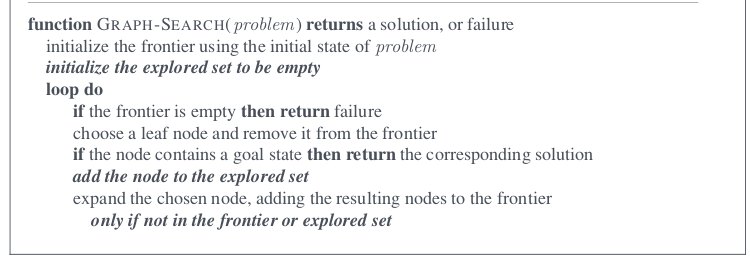
\includegraphics[width=1\linewidth]{./images/code-grafo.png}
  \caption{Esempio di ricerca del cammino minimo per Bucharest con grafo.}
   \label{fig: esempio-ricerca-grafo}
\end{figure}
\noindent
\begin{figure}[H]
\centering
  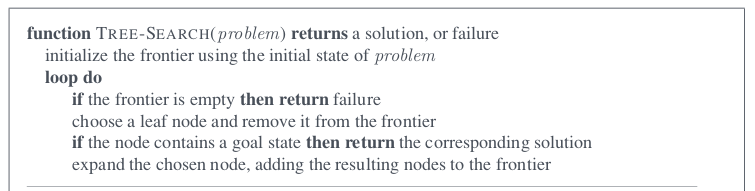
\includegraphics[width=1\linewidth]{./images/code-albero.png}
  \caption{Esempio di ricerca del cammino minimo per Bucharest con albero.}
   \label{fig: esempio-ricerca-albero}
\end{figure}
\noindent
\end{document}